\chapter{Figures}
In \LaTeX, integrating figures is a straightforward process. To insert them, you should utilise the environment \verb|\begin{figure}|. You can customise the \verb|width| parameter according to your requirements, but it is crucial to select a high-quality figure when inserting it into your documents. It is equally crucial to furnish a well-crafted caption. If necessary, consider including citations or references to indicate the figure's origin. The caption environment is denoted as \verb|\caption{TEXT}|. However, to generate a smaller caption for the Table of Figures, be sure to utilise the format \verb|\caption[SMALL_TEXT]{BIG_TEXT}|. By following the aforementioned tips, we can create a figure as demonstrated in \autoref{fig:figure-01}.

\begin{figure}[!htpb]
    \centering
    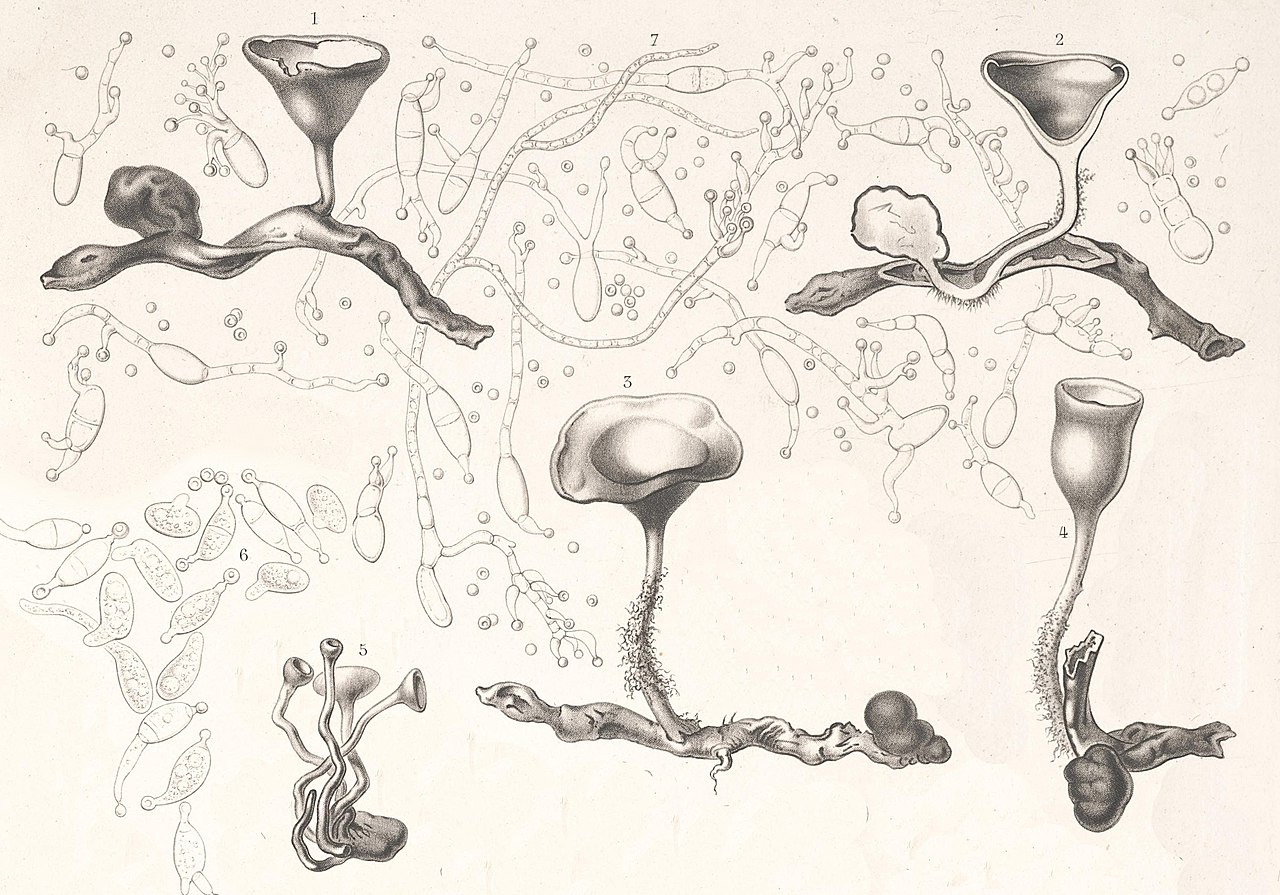
\includegraphics[width=\linewidth]{Figures/PezizaTuberosa.jpg}
    \caption[Illustration of the fungus Dumontinia tuberosa]{Illustration of the fungus Dumontinia tuberosa by physician, mycologist, and illustrator Charles Tulasne (1816–1884) in the book Selecta Fungorum Carpologia (1861–65). (Name of the original work: Peziza tuberosa parasite on Anemone nemorosa)}
    \label{fig:figure-01}
\end{figure}

\section{Side-by-Side Figures}
For the purpose of comparing or for other reasons, you can insert side-by-side figures using both the \verb|\begin{figure}| and \verb|\begin{subfigure}| environments. You can also refer to the sub-figure as \autoref{fig:figure-02.1} and \autoref{fig:figure-02.2}.

\begin{figure}[!htpb]
    \centering
    \begin{subfigure}{0.45\textwidth}
        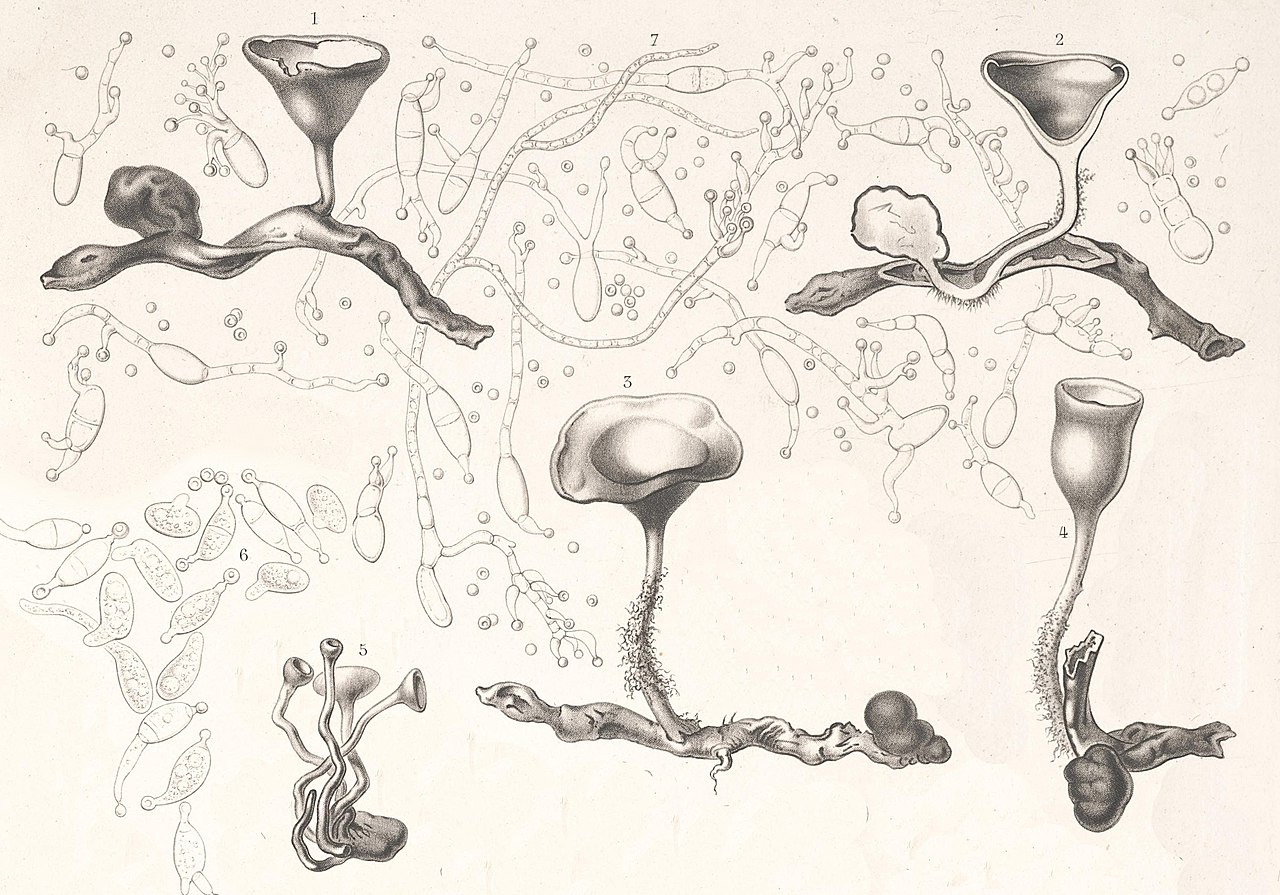
\includegraphics[width=\textwidth]{Figures/PezizaTuberosa.jpg}
        \caption{Caption for Image 1}
        \label{fig:figure-02.1}
    \end{subfigure}
    \hspace{.5cm} % Adjust the space as needed
    \begin{subfigure}{0.45\textwidth}
        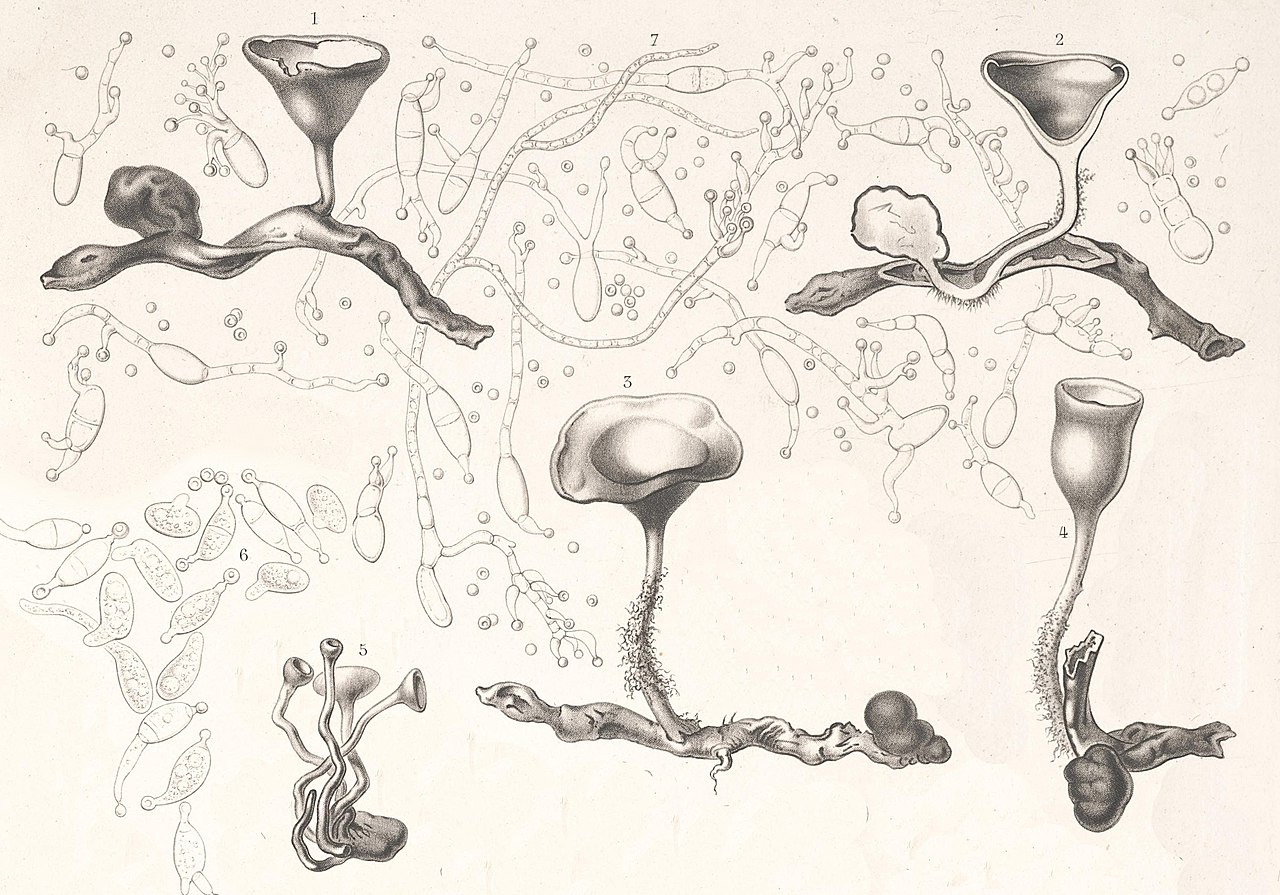
\includegraphics[width=\textwidth]{Figures/PezizaTuberosa.jpg}
        \caption{Caption for Image 2}
        \label{fig:figure-02.2}
    \end{subfigure}
    \caption{Overall Caption for the Figure}
    \label{fig:figure-02}
\end{figure}

To customise the spacing between sub-figures, utilise the \verb|\hspace{VALUE}| command. Establishing adequate spacing is crucial for enhancing visual appeal and ensuring a reader-friendly experience. Below is a code snippet that represents the \autoref{fig:figure-02} - both label and caption text were omitted.

\begin{verbatim}
\begin{figure}[!htpb]
    \centering
    \begin{subfigure}{0.45\textwidth}
        \includegraphics[width=\textwidth]{FIGURE_PATH}
        \caption{TEXT}
        \label{TEXT}
    \end{subfigure}
    \hspace{.5cm} % Adjust the space as needed
    \begin{subfigure}{0.45\textwidth}
        \includegraphics[width=\textwidth]{FIGURE_PATH}
        \caption{TEXT}
        \label{TEXT}
    \end{subfigure}
    \caption{TEXT}
    \label{TEXT}
\end{figure}
\end{verbatim}